\documentclass[crop,tikz]{standalone}

\usepackage[utf8]{inputenc}
\usepackage{tikz-qtree}

\begin{document}
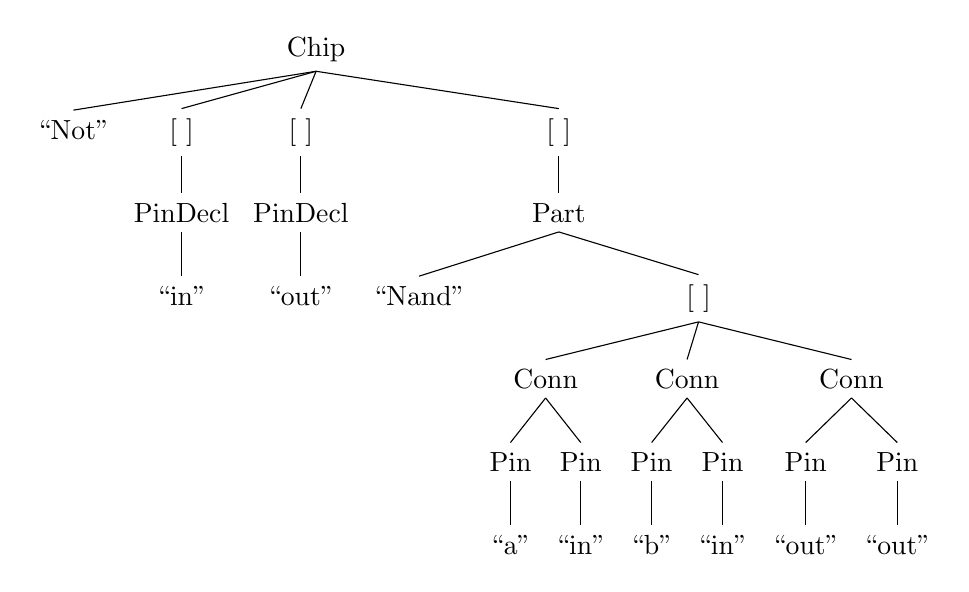
\begin{tikzpicture}
  \Tree [.Chip “Not”
    [.[\ ]
      [.PinDecl “in” ]
    ]
    [.[\ ]
      [.PinDecl “out” ]
    ]
    [.[\ ]
      [.Part “Nand”
        [.[\ ]
          [.Conn
            [.Pin “a” ]
            [.Pin “in” ]
          ]
          [.Conn
            [.Pin “b” ]
            [.Pin “in” ]
          ]
          [.Conn
            [.Pin “out” ]
            [.Pin “out” ]
          ]
        ]
      ]
    ]
  ]
\end{tikzpicture}
\end{document}
